\appendix

\section{Detectability, power, and interval estimates}
\label{app:power}

This appendix reports the three quantities defined in Section~\ref{sec:power}
for every association tested in this paper. All of them are computed from the
per-checkpoint results already reported in Section~\ref{sec:results}: no
checkpoint is re-evaluated, no model is retrained, and no additional data are
used.

\subsection{What the designs could have detected}
\label{app:power-design}

Two permutation designs are used in this paper and they are not
interchangeable. Design~A is continuous--continuous (a geometry metric against
Mahalanobis AUROC, $n = 13$, tie-free), and its exact null runs over all $13!$
orderings. Design~B tests an ordinal dose against a value (a geometry metric,
scorer AUROC, or probe AUROC against $\lambda_{\mathrm{orth}}$), where the dose
is tied by construction and the exact null runs over the $72{,}072$ distinct
label arrangements consistent with the 5/5/3 rung counts, or the $1{,}680$
arrangements of the 3/3/3 common-seed subset. Table~\ref{tab:power-design}
gives $\tau_{\mathrm{crit}}$, the attainable maximum $|\tau|$, and power for
each; Figure~\ref{fig:power}(A) shows the full power curves.

Design~B's attainable maximum is $0.840$ rather than $1.000$ because a tied
predictor caps $\tau_b$ below unity: with 5/5/3 rung sizes, a perfectly
monotone ladder --- every checkpoint at a lower $\lambda_{\mathrm{orth}}$
ranked below every checkpoint at a higher one --- yields exactly $\tau_b =
0.840$. The condition-number result of Section~\ref{sec:geometry-changes}
attains that ceiling.

% generated by analysis/make_tables_power_tmlr.py from
% results/power_design_summary.csv -- do not edit by hand.
\begin{table}[t]
\centering
\caption{Detectability of the two permutation designs used in this study.
Design~A is the continuous--continuous test of a geometry metric against
Mahalanobis AUROC (Section~\ref{sec:geometry-auroc}); Design~B is the ordered
ladder used for every test against $\lambda_{\mathrm{orth}}$
(Sections~\ref{sec:geometry-changes}, \ref{sec:generalizes} and
\ref{sec:decodable}). ``Null space'' is the number of distinct label
arrangements enumerated for the exact test.
$\tau_{\mathrm{crit}}$ is the smallest $|\tau|$ attainable at that design whose
two-sided exact permutation $p$-value reaches $0.05$: no dataset, however clean,
can produce a significant association below it. Power is computed by simulation
($2\times10^{4}$ datasets per grid point, common random numbers) under an
alternative whose expected value of the reported statistic equals the stated
$\tau$ --- bivariate normal for Design~A, a linear dose shift
$y = \theta d + \varepsilon$ for Design~B. MDE$_{80\%}$ is the expected $\tau$ at
which power first reaches $0.80$.}
\label{tab:power-design}
\footnotesize
\begin{tabular}{lccccccc}
\toprule
 & & Null & Max. & & \multicolumn{2}{c}{Power at} & \\
\cmidrule(lr){6-7}
Design & $n$ & space & $|\tau|$ & $\tau_{\mathrm{crit}}$ & $\tau=0.3$ & $\tau=0.5$ & MDE$_{80\%}$ \\
\midrule
A: continuous--continuous & 13 & $13!$ & 1.000 & 0.436 & 0.27 & 0.71 & 0.54 \\
B: 5/5/3 ordered ladder & 13 & 72,072 & 0.840 & 0.473 & 0.23 & 0.63 & 0.57 \\
B: 3/3/3 common-seed subset & 9 & 1,680 & 0.866 & 0.609 & 0.14 & 0.39 & 0.69 \\
\bottomrule
\end{tabular}
\end{table}


\subsection{What the data exclude}
\label{app:power-ci}

Table~\ref{tab:tau-ci} gives a 95\% bias-corrected and accelerated (BCa)
bootstrap interval \citep{efron1987better} for every $\tau$ reported in the
paper, over $2\times10^{4}$ resamples drawn \emph{within} rung so that the
5/5/3 design is held fixed; $\lambda_{\mathrm{orth}}$ is a fixed design factor,
not a sampled one, and resampling across rungs would bootstrap a quantity this
experiment never estimated. Figure~\ref{fig:power}(B) plots the same intervals
against the two designs' critical values.

Resampling with replacement necessarily creates ties in a response that was
tie-free as observed, and the two standard tie treatments pull an interval in
opposite directions: the $\tau_b$ denominator $\sqrt{(n_0 - t_x)(n_0 - t_y)}$
shrinks as ties accumulate and so inflates $|\tau|$ on tied resamples, whereas
the design-normalized form $(2J - M)/\sqrt{M n_0}$ pins the denominator to the
original design and cannot exceed the design ceiling. The two are identical on
the observed data. Both were computed; over the tests reported here their endpoints
differ by a median of $0.027$ and at most $0.091$, and the two agree on every
$|\tau| = 0.3$ exclusion verdict, so no statement in this paper depends on the
choice. Table~\ref{tab:tau-ci}
reports the $\tau_b$ version.

One case admits no valid interval. Where an observed $\tau$ attains the maximum
its design permits --- condition number against $\lambda_{\mathrm{orth}}$,
$\tau = 0.840$ --- every resample lies at or below the observed value, the
resampling distribution is one-sided by construction, and a nominal interval
computed from it can fail even to contain its own point estimate. That case is
reported as a point without an interval, and its exact permutation $p$-value is
the meaningful inference.

% generated by analysis/make_tables_power_tmlr.py from
% results/kendall_tau_ci.csv -- do not edit by hand.
\begin{table}[t]
\centering
\caption{Every Kendall's $\tau$ reported in this paper with a 95\% bootstrap
confidence interval ($2\times10^{4}$ stratified resamples, bias-corrected and
accelerated; resampling is within-rung, so the 5/5/5 design is held fixed).
``Largest $|\tau|$ not excluded'' is the interval endpoint furthest from zero:
the effect size each non-significant result still permits.}
\label{tab:tau-ci}
\small
\begin{tabular}{lccc}
\toprule
Test & $\tau$ & 95\% CI & Largest $|\tau|$ not excluded \\
\midrule
\multicolumn{4}{l}{\emph{Geometry metric vs.\ $\lambda_{\mathrm{orth}}$ (Section~\ref{sec:geometry-changes})}} \\
\addlinespace[0.15em]
\quad Condition number & $\phantom{-}0.845$ & \multicolumn{2}{c}{at design ceiling --- see note} \\
\quad Fisher ratio (Hotelling--Lawley) & $\phantom{-}0.237$ & $[-0.335,\ \phantom{-}0.612]$ & 0.61 \\
\quad Fisher ratio (decoupled scalar) & $\phantom{-}0.237$ & $[-0.313,\ \phantom{-}0.612]$ & 0.61 \\
\quad Mardia's kurtosis ($b$) & $\phantom{-}0.056$ & $[-0.313,\ \phantom{-}0.385]$ & 0.38 \\
\quad Mardia's kurtosis ($z$) & $\phantom{-}0.011$ & $[-0.344,\ \phantom{-}0.363]$ & 0.36 \\
\addlinespace
\multicolumn{4}{l}{\emph{Geometry metric vs.\ Mahalanobis AUROC (Section~\ref{sec:geometry-auroc})}} \\
\addlinespace[0.15em]
\quad Condition number & $\phantom{-}0.143$ & $[-0.253,\ \phantom{-}0.440]$ & 0.44 \\
\quad Fisher ratio (Hotelling--Lawley) & $-0.276$ & $[-0.663,\ \phantom{-}0.216]$ & 0.66 \\
\quad Fisher ratio (decoupled scalar) & $-0.219$ & $[-0.629,\ \phantom{-}0.286]$ & 0.63 \\
\quad Mardia's kurtosis ($b$) & $-0.086$ & $[-0.490,\ \phantom{-}0.339]$ & 0.49 \\
\quad Mardia's kurtosis ($z$) & $-0.067$ & $[-0.460,\ \phantom{-}0.329]$ & 0.46 \\
\addlinespace
\multicolumn{4}{l}{\emph{Directed scorer AUROC vs.\ $\lambda_{\mathrm{orth}}$ (Section~\ref{sec:generalizes})}} \\
\addlinespace[0.15em]
\quad Mahalanobis & $\phantom{-}0.192$ & $[-0.311,\ \phantom{-}0.572]$ & 0.57 \\
\quad Cosine-to-centroid & $\phantom{-}0.372$ & $[-0.151,\ \phantom{-}0.685]$ & 0.68 \\
\quad $k$-NN ($k=1$) & $\phantom{-}0.146$ & $[-0.391,\ \phantom{-}0.589]$ & 0.59 \\
\quad $k$-NN ($k=10$) & $\phantom{-}0.214$ & $[-0.358,\ \phantom{-}0.611]$ & 0.61 \\
\quad $k$-NN ($k=50$) & $\phantom{-}0.304$ & $[-0.192,\ \phantom{-}0.658]$ & 0.66 \\
\addlinespace
\multicolumn{4}{l}{\emph{Domain-probe AUROC vs.\ $\lambda_{\mathrm{orth}}$ (Section~\ref{sec:decodable})}} \\
\addlinespace[0.15em]
\quad Logistic regression & $\phantom{-}0.259$ & $[-0.199,\ \phantom{-}0.612]$ & 0.61 \\
\quad Linear SVM & $\phantom{-}0.304$ & $[-0.152,\ \phantom{-}0.621]$ & 0.62 \\
\quad Random forest & $\phantom{-}0.192$ & $[-0.315,\ \phantom{-}0.543]$ & 0.54 \\
\bottomrule
\end{tabular}

\vspace{0.25cm}
\begin{minipage}{\textwidth}
% undo the \centering of the enclosing table, so the note sets as a paragraph
\leftskip=0pt \rightskip=0pt \parfillskip=0pt plus 1fil
\small \emph{Note.} Condition number vs.\ $\lambda_{\mathrm{orth}}$ attains
$\tau = 0.845$, the maximum value the 5/5/5 design permits (a perfectly monotone
ladder). Every bootstrap resample therefore lies at or below the observed value,
the resampling distribution is one-sided by construction, and no bootstrap
interval is valid; the exact permutation $p$-value ($p = 2.6 \times 10^{-6}$) is the
meaningful inference for that effect. Of the seventeen non-significant
associations, none has an interval that excludes $|\tau| = 0.3$.
\end{minipage}
\end{table}


\begin{figure}[t]
\centering
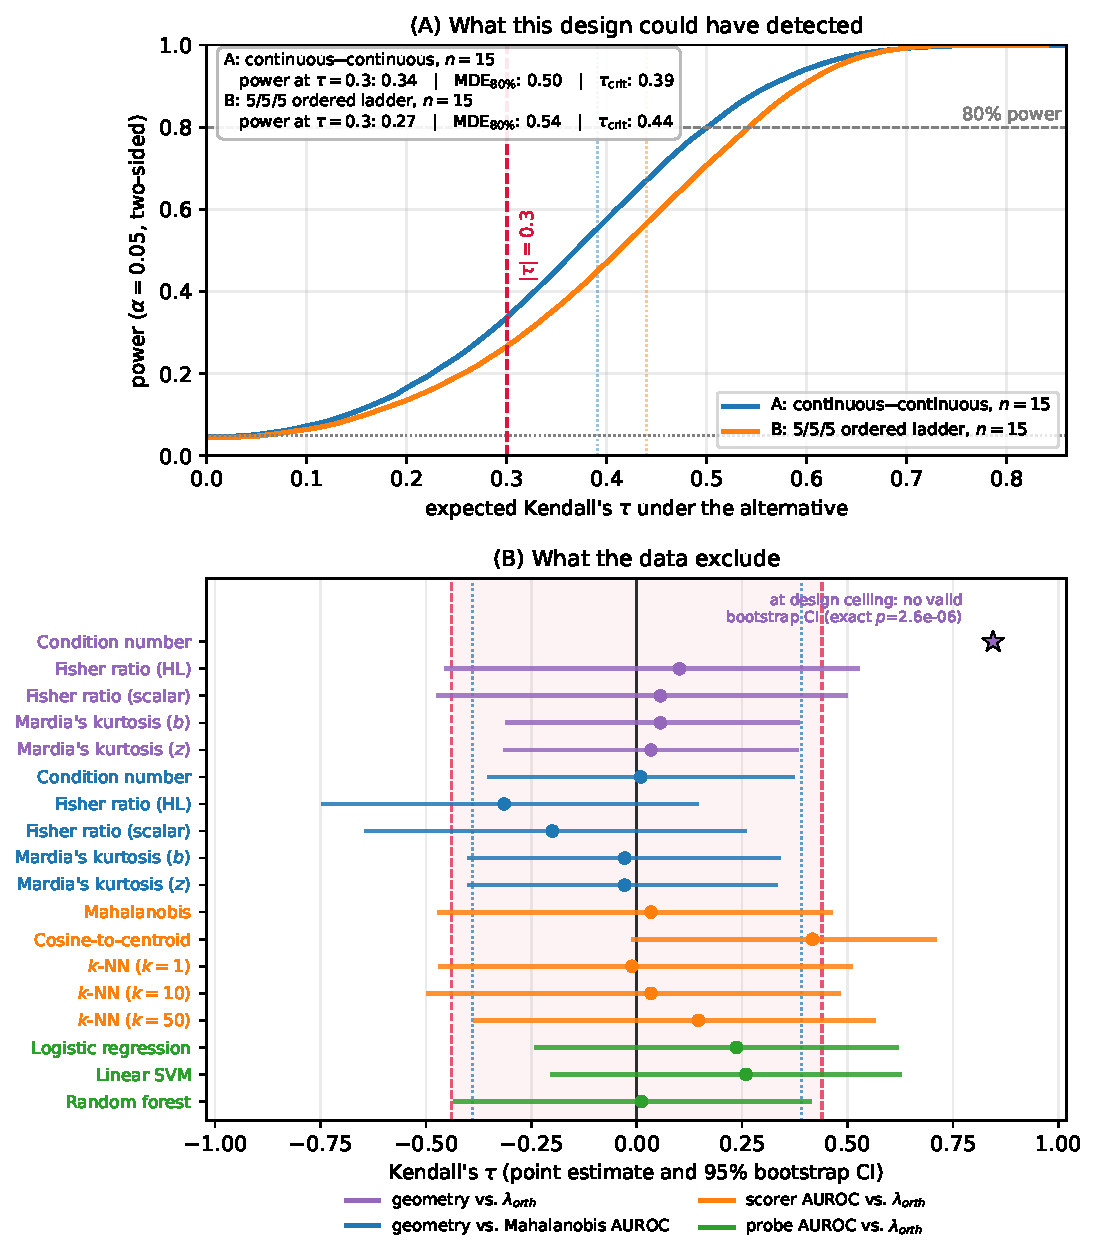
\includegraphics[width=0.93\linewidth]{figs/fig7_power.pdf}
\caption{Effect-size and power bounds on this study's non-significant
associations (exact permutation tests, $\alpha = 0.05$). (A) Power against the
expected value of the reported statistic, for the three designs of
Table~\ref{tab:power-design}; vertical dotted lines mark each design's
$\tau_{\mathrm{crit}}$ and the dashed red line marks $|\tau| = 0.3$, the effect
size fixed in the analysis plan (Section~\ref{sec:stats}). That value lies below
every $\tau_{\mathrm{crit}}$, so the plan's conjunction of $|\tau| \geq 0.3$
with significance at $\alpha = 0.05$ was unsatisfiable at these designs.
(B) Observed Kendall's $\tau$ with 95\% BCa bootstrap intervals for all
eighteen association tests reported in the paper. The shaded band spans
$\pm\tau_{\mathrm{crit}}$ for the 5/5/3 ladder (dashed bounds); dotted bounds
mark the continuous--continuous design. Condition number against
$\lambda_{\mathrm{orth}}$ (star) sits at its design ceiling and is drawn without
an interval, for the reason given in Section~\ref{app:power-ci}.}
\label{fig:power}
\end{figure}
